\documentclass{sig-alternate} % sets document style to sig-alternate
% packages
% typesetting
\usepackage{amsmath}
% \usepackage{hanging} % hanging paragraphs with \hanging, like in references. doesn't translate to HTML
\usepackage[pdfpagelabels=false]{hyperref} % produce hypertext links, includes backref and nameref
\usepackage{microtype} % better typography
% \usepackage{textcomp} % for better tildes
% \newcommand{\texttildemid}{\raisebox{0.4ex}{\texttildelow}} % creates a text mid tilde, a low tilde moved up
\usepackage{textgreek}
\usepackage{xurl} % defines url linebreaks, loads url package
% layout
\usepackage{calc} % so we can do inline math within \setlength
\usepackage{enumitem} % control layout of itemize, enumerate, description
\usepackage{fancyhdr} % control page headers and footers
% \usepackage{float} % improved interface for floating objects, adds H float
% \usepackage{multicol} % intermix single and multiple column pages
% language
\usepackage[english]{babel} % multilanguage support
\usepackage[utf8]{inputenc} % utf8 encoding, wider character set
% \usepackage{textgreek} % typeset greek letters in text mode
% misc
\usepackage{authblk} % support for footnote style author/affiliation
\usepackage[backend=biber, style=apa]{biblatex} % sophisticated bibliographies % necessary for HTML to display author info and date on abstract page
\usepackage{csquotes} % advanced quotations, makes biblatex happy
\usepackage{graphicx} % builds upon graphics package, \includegraphics
\usepackage{xcolor} % color extensions
% tables and figures
\usepackage{caption} % customize captions in figures and tables (rotating captions, sideways captions, etc)
%\usepackage{cuted} % allow mixing of \onecolumn and \twocolumn on same page
\usepackage{multirow} % create tabular cells spanning multiple rows
%\usepackage{subfigure} % deprecated, support for manipulation of small figures
\usepackage{tabularray} % better table construction, does not translate to HTML
\UseTblrLibrary{varwidth}
% dummy text
\usepackage{lipsum} % lorem ipsum dummy text

\setlength{\paperheight}{11in} % sets document height, prevents warning

\pagestyle{fancy} % sets pagestyle to fancy for fancy headers and footers. remember to change the header depending on article type
% allows the header to take the full width of the page, doesn't work with XeLaTeX or LuaLaTeX (?) https://www.reddit.com/r/LaTeX/comments/awtrb2/how_to_you_make_the_headerfooter_extend_the/
\newlength{\oddmarginwidth}
\setlength{\oddmarginwidth}{1in+\hoffset+\oddsidemargin}
\newlength{\evenmarginwidth}
\setlength{\evenmarginwidth}{\evensidemargin+1in}
\fancyhfoffset[LO,RE]{\oddmarginwidth}
\fancyhfoffset[LE,RO]{\evenmarginwidth}

% header and footer
% modern way to set header image, using fancyhdr
\renewcommand{\headrulewidth}{0pt} % defines thickness of line under header
\renewcommand{\footrulewidth}{0pt} % defines thickness of line above header
\setlength\headheight{80.0pt} % sets height between top margin and header image, effectively moves page contents down
\addtolength{\textheight}{-80.0pt} % seems to affect the lower height. maybe only works properly if footer numbers enabled?
\fancyhf{}
\fancyhead[CE, CO]{
\includegraphics[width=\pdfpagewidth]{headerImage.png}}

\hypersetup{colorlinks=true,urlcolor=blue} % sets link color to blue
\urlstyle{same} % sets url typeface to same as rest of text

% set caption and figure to italics, label bold, left align captions, does not transfer to HTML
\captionsetup{labelfont=bf, font={large, it}, justification=raggedright, singlelinecheck=false}
\renewcommand\theContinuedFloat{\alph{ContinuedFloat}} % has something to do with subfigures... don't remember why i used it

% this next bit is confusing, but essentially changes the width of the abstract. Seems to have been copied from this https://tex.stackexchange.com/questions/151583/how-to-adjust-the-width-of-abstract
\let\oldabstract\abstract
\let\oldendabstract\endabstract
\makeatletter %changes @ catcode to enable modification (in parsep)
\renewenvironment{abstract} % alters the abstract environment
{\renewenvironment{quotation}% alters the quotation environment in the abstract environment ?
               {\list{}{\addtolength{\leftmargin}{1em} % change this value to add or remove length to the the default ?
                        \listparindent 1.5em%
                        \itemindent    \listparindent%
                        \rightmargin   \leftmargin%
                        \parsep        \z@ \@plus\p@}%
                \item\relax}%
               {\endlist}%
\oldabstract}
{\oldendabstract}
\makeatother %changes @ catcode to disable modification

\begin{document}
\title{Sensemaking Opportunities for Students Experiencing Difficulty: A Mixed Methods Study}

\author[1]{\large \color{blue} Rachel Juergensen} % make sure there are no spaces after the author's name
\author[2]{\large \color{blue} Delinda van Garderen} % make sure there are no spaces after the author's name


\affil[1]{Delaware State University}
\affil[2]{University of Missouri - Columbia}
\toappear{} % the sig.alternate document type includes a copyright warning that appears at the bottom of the first page. This makes that not appear/be empty. Don't ask my why it's there in the first place /shrug

\maketitle % prints article title
\begin{@twocolumnfalse} 
\begin{abstract}
\item %the abstract is a quotation and a list, so this must be an item
\begin{large}
\textit{All students deserve to be engaged in high-quality science instruction that moves beyond memorization and recall of facts and offers opportunities for sensemaking. Science achievement is alarmingly low signifying there is a large percentage of students experiencing difficulty in science. The low science achievement may be symptomatic of gaps in opportunities for sensemaking within the science classroom. Using an explanatory sequential mixed methods design, the current study explored the relationship between middle school science teacher beliefs and opportunities students experiencing difficulty in science had to participate in sensemaking discussions. Integrated findings from the study suggest that teachers’ beliefs influenced the opportunities students experiencing difficulty had to participate in sensemaking discussions and, at times, there was a mismatch between teacher beliefs and practice. The current study addresses an important gap in the research literature on opportunities students experiencing difficulty have for sensemaking in science classrooms, a grossly under researched area of inquiry.}
\item Keywords: Science, Students with disabilities, Sensemaking, Beliefs, Equity

\end{large}     
\end{abstract}
\end{@twocolumnfalse}

%% AUTHOR INFORMATION
\textbf{*Corresponding Author, Rachel Juergensen}\\ % corresponding author
\href{mailto:rjuergensen@desu.edu}{(rjuergensen@desu.edu)} \\ % author email
\textit{Submitted Jul 17 2025} \\ % submitted date
\textit{Accepted Aug 12 2025} \\ % accepted date
\textit{Published Online MMM DD YYYY} \\ % published online date, updated after author approval
\textit{DOI: } \\ % doi, updated after author approval, in spreadsheet on server
\pagebreak 
\clearpage % both needed to go to next page
\begin{large}

\section*{INTRODUCTION}

Despite the push for improvement in science achievement for all students by researchers and policy makers (e.g., National Research Council, 2013; U.S. Department of Education, 2019), there is still notably low achievement in the content area of science, especially when compared to other content areas such as mathematics and reading (NGSS Lead States, 2013; U.S. Department of Education, 2019). On the 2019 National Assessment of Educational Progress (NAEP) Science Assessment, 65\% of students who performed basic or below basic (not proficient) on the NAEP Science Assessment. The achievement gap between students proficient in science and students not proficient in science is troubling. 

Findings from research suggest the gaps in achievement are largely a result of the inequitable learning opportunities students receive within science (Moss et al., 2008; National Research Council, 2012; Oakes et al., 1990). For example, some students receive more opportunities to participate in whole-class discussions than others. Opportunities to participate in learning through whole-class discussion is critical as Vygotsky (1978) suggests that communication is a pre-requisite to learning and understanding concepts. Furthermore, when science learning includes mediation through instruction that includes discussion, students experiencing difficulty not only benefit but can approach the level of learning of their peers who are not experiencing difficulty (Mastropieri et al., 1998; Scruggs et al., 1993). Oakes and colleagues (1990) go on further to say, “unequal learning opportunities provide some specific clues to how educational practices may help create and perpetuate differences in achievement and participation” (p. 6). Pak and Parsons (2020) take it a step further to describe what is happening in terms of the gap as an equity gap and stress that the current educational system underserves students who may be experiencing difficulty. 

National organizations such as the National Science Teaching Association (NSTA) and the National Science Foundation (NSF) promote equitable instructional opportunities for all students (Anderson et al., 1998). National science standards like the Next Generation Science Standards (NGSS) were developed for \textit{all} students to have equitable access to more rigorous science instruction (NGSS Lead States, 2013). Additionally, the Every Student Succeeds Act (ESSA; Every Student Succeeds Act, 2015) requires that all students be taught to high academic standards and states a commitment to equal opportunity for all students. National organizations, national standards, and current law are all promoting, and in some cases requiring, equitable opportunities to learn for all students but there is currently little research suggesting to what extent these opportunities are or are not occurring within the science classroom for students experiencing difficulty in science. The term “students experiencing difficulty” is used rather than “students who struggle” to signify that their difficulty or struggle is not fixed, does not define them as a student, but is simply an experience they are having that has the potential to change. Therefore, it is critical to look beyond simply \textit{if} opportunities to learn are provided and to look more deeply at what types of opportunities are made available and who is or is not receiving these opportunities (Miller et al., 2018). Pak and Parsons (2020) argue that to study instructional practices gaps in equity must be explicitly examined. Additionally, they argue that systemic and individual biases toward students experiencing difficulty need to be addressed to move toward transformational practices within more rigorous curricula. The priority then, and the purpose of this study, is to examine equity issues, namely sensemaking opportunities within whole-class discussions, during science instruction for students experiencing difficulty in science.

\section*{REVIEW OF THE LITERATURE}

\subsection*{Sensemaking}

Odden and Russ (2019) define sensemaking as “a dynamic process of building or revising an explanation in order to “figure something out”—to ascertain the mechanism underlying a phenomenon in order to resolve a gap or inconsistency in one's understanding” (p. 192). Going public with ideas, modeling, and reasoning from evidence are all a large part of the NGSS and critical to sensemaking (NGSS Lead States, 2013). Having regular and meaningful opportunities to engage in sensemaking practices is critical to fostering equitable participation in science and teachers play a critical role in who gets opportunities and what those opportunities look like (Kloser et al., 2019).

\subsubsection*{Teachers’ Role in Sensemaking Opportunities}

When teachers are at the center of facilitating student talk, they are at the center of facilitating sensemaking. In their review of student sensemaking across disciplines, Fitzgerald and Palincsar (2019), found several teaching practices that promote sensemaking. Overarching all the practices was engagement in discourse. Within discourse, they highlighted several teaching practices associated with sensemaking including, questioning, making connections, increasing challenge, enculturating students to engage in sensemaking, and differentiating instruction, all of which fall within the role of the teacher. Drew and Thomas (2021) suggest engaging students in discussion where all students are expected to listen and speak. They go on further to say that discussion is an area that students experiencing difficulty may struggle so teachers need to ensure students are explicitly taught how to participate in discussions. Furthermore, in science classrooms, teachers hold the power to engage students in the discourse taking place (Kelly, 2007) and a teachers’ interactions with students have the power to influence student engagement in sensemaking (Mercer et al., 2009; Resnick et al., 2010). However, a teachers’ interaction with students is influenced by their beliefs (Kiely et al., 2015).

\subsection*{Teachers’ Beliefs}

Teachers’ beliefs are just a small part of a more complex system (Churchland \& Churchland, 2013; Fives \& Buehl, 2012). Research suggests that overall, teachers’ beliefs influence their practice including what they do in the classroom, who they interact with, and how they interact with students (Cain \& Cain, 2012; Khader, 2012; Klehm, 2014; Phipps \& Borg, 2009).

Empirical evidence suggests that teachers’ beliefs may impact the instructional interactions that take place, and the level of dialogue teachers use with students (Jordan et al., 1993; Jordan \& Stanovich, 2003; Kahn \& Lewis, 2014; Stanovich \& Jordan, 1998). To echo this, Klehm (2014) found that teachers’ beliefs about students’ ability to learn and ability to achieve higher level thinking, such as the thinking required by the NGSS, predicted scores on achievement tests. Said another way, teachers’ beliefs have an impact on their teaching practices and therefore, the achievement of their students. Assessing teachers’ beliefs can show whether teachers are more likely to engage students experiencing difficulty in more cognitively demanding instruction (Kiely et al., 2015) such as the instruction required by the NGSS. Research suggests that students experiencing difficulty are often given less access to demanding science instruction (Weiss et al., 2003) and teachers hold low expectations for their learning and performance (Cook et al. 2000; Moss et al., 2008; Pettit, 2011) which can impact their outcomes (Jussim \& Harber, 2005). Whether or not a student experiencing difficulty gets the support they need in the classroom has connections to a teacher’s beliefs (Kiely et al., 2015).

\section*{RATIONALE}

The NGSS state that all students are capable of sensemaking in science and stress the criticality of providing students with equitable opportunities to engage in sensemaking in science classrooms (Lee et al., 2014). Research suggests the teacher plays a critical role in who gets opportunities for sensemaking and what those opportunities look like in science classrooms.  However, there is little research looking specifically at students experiencing difficulty in the science classroom. We cannot say \textit{science for all} if we do not know if \textit{all} includes students experiencing difficulty. Therefore, the purpose of this study is to explore equity issues, namely sensemaking opportunities during whole-class discussions, for this group of students. The following research questions will be addressed: 

% change enumerate for html version

\begin{enumerate}[leftmargin = 1in]
    \item[Quant RQ1:] Is there a significant relationship between student group and opportunities to participate in sensemaking discussions?
    \item[Qual RQ2:] What are teachers’ beliefs about students experiencing difficulty and opportunities for sensemaking in science?
\end{enumerate}
\newpage
\begin{enumerate}[leftmargin = 1in]
    \item[MIXED RQ3:] What is the relationship between teacher beliefs about students experiencing difficulty and opportunities to participate in sensemaking discussions?
\end{enumerate}

\section*{METHODS}

\subsection*{Research Design}
The current study used an explanatory sequential mixed methods design (Figure 1; Creswell \& Plano Clark, 2018). This research design was well suited for the current study because it allowed for the use of qualitative data to further explain the quantitative results. 

\begin{figure}[htb]
    \centering
    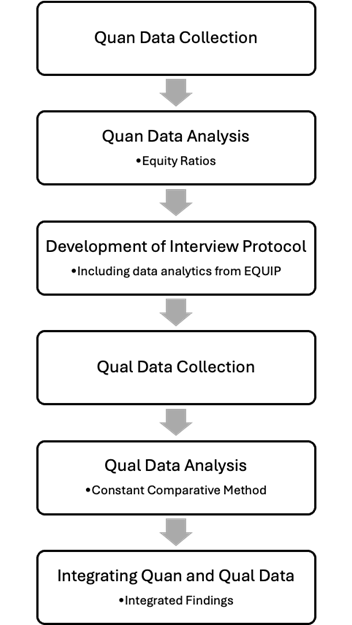
\includegraphics[width=0.75\linewidth]{images/fig1crop.png}
    \caption{Explanatory Sequential Study Design}
\end{figure}

\subsection*{Participants}

Teachers recruited for this study were aware they were participating in a study focused on examining opportunities for sensemaking in the context of whole-class discussions. Teacher participants (\textit{n} = 3) represented two districts in the Midwest. All three teacher participants are general education science teachers at the middle school level. See Table 1 for detailed teacher participant demographics. 

\begin{table*}[thb]
\caption{Demographic Information of Teacher Participants}
\begin{tabular}{ccccccc}
\hline
Teacher & District & Experience & Grade & Highest Degree Earned & Race & Gender \\ \hline
A & 2 & 3 & 8 & MEd Admin & white & female \\
B & 1 & 24 & 6 & MEd English (TESOL) & white & female \\
C & 2 & 14 & 7 & MEd (C\&I) & white & female \\ \hline
\end{tabular}
\end{table*}

After classroom observations (described below), teachers were asked to sort their students (\textit{n} = 52) into one of two student groups: 1) students experiencing difficulty in science and 2) students NOT experiencing difficulty in science. Twenty-five percent (\textit{n} = 13) of the student participants were identified as students experiencing difficulty in science. This included both students with and without Individual Education Programs (IEPs). Given that a focus of the study was on teacher beliefs (i.e., who experiences difficulty and how that influences their interactions in the classroom) and would be elaborated on as a part of the data collection, the teachers were not provided with a definition of who a student is that experiences difficulty in science. The decision was made by teachers based on formative assessments, summative assessments, or observations made during science instruction throughout that school year. It was important that teachers were the ones identifying students experiencing difficulty in science as they were the ones who spent the most time interacting with this group of students. According to Reinholz and Shah (2018) it is logical to have teachers identify the students experiencing difficulty because the ways teachers identify students are what drives the interactions they have with students and ultimately the opportunities they have during instruction. Teacher participants were asked to give a rationale for why they identified a student as experiencing difficulty in science and gave the following reasons: trouble focusing, executive functioning issues, low work ethic, low self-esteem, poor reading and writing skills, low attendance, task completion issues, challenges with working independently, struggling with science concepts, and suspected undiagnosed dyslexia. 

\subsection*{Instructional Units}

Across all three units selected by the teachers, they used whole-class discussions as a way for students to engage in sensemaking. 

Teacher A’s unit focused on human body systems. She began by focusing on each system independently and spent time helping students make sense of the organs and the functions of the organs. Then, she began to ask students to think about the ways the body systems worked together. She did this by using modeling and helping the students make connections to their own bodies. She stated that this content was critical because so many of her students had future plans to be nurses or work in the medical field. 

Teacher B’s unit focused on climate change. She focused heavily on getting her students to make claims backed by evidence and reasoning. Teacher B wanted her students to be able to decide if evidence was valid and think about ways they could cope with future climate change. In addition to the goal of making claims backed by evidence and reasoning, she wanted her students to be able to write about their claims in a way that they could be shared with and critiqued by other students. 

Teacher C’s unit focused on Earth science and the human body. Specifically, she focused on climate and how the climate effects human body systems. Her goals for students were to have a deeper understanding of climate including the why and how of climate, how geographic features affect climate, how people affect climate, and how the climate affects people. 

\subsection*{Quantitative Phase}

The goal of the quantitative phase was to examine equity issues by comparing the opportunities students experiencing difficulty received during whole-group science discussions to their peers who were not experiencing difficulty. Classroom observations of each lesson within one whole unit were conducted with all three teachers. A total of 23 lessons were observed across all three teacher participants.

Audio from each observation was transcribed and then checked for accuracy by the principal investigator. After all transcriptions were accurate, a total of 26 whole-class discussions were identified. Whole-class discussions were identified as instructional time where the whole-class was involved in a discussion. Students and the teacher needed to be actively discussing science content, phenomena, or a lab. Whole-class discussions did not include independent work or small group work. 

Within each whole-class discussion, a total of 428 participation sequences were identified. For this study, participation sequences served as the unit of analysis. A participation sequence is any string of utterances from a single student. Meaning, if a new student contributes, a new string of utterances or participation sequence begins. If a student speaks back and forth with the teacher and no other student contributes, then this is all considered part of one string of utterances or participation sequence. Several instances were not counted as a participation sequence including non-consenting or unidentifiable students speaking, multiple students answering or choral responses, and side conversations or turn and talks. Only whole-class discussion with \textit{visible participation} was included as a participation sequence. The purpose for these decisions was it allowed for the data to be disaggregated by student group, it showed multiple back-and-forth moves which reflect discussion moves teachers use in classroom instruction, and segmenting when a new student speaks made it easier to identify new participation sequences. Further, focusing only on whole-class discussions that were visible allowed student participation to be seen by other students which contributes to positioning students as sensemakers within the discussion. 

\subsubsection*{Quantitative Data Coding}

Participation sequences were organized onto a spreadsheet which included the participation sequence number, speaker name, the transcript of what was said, and a column for each code. Audio recordings were also available to coders if needed for review. The participation sequences were coded among three dimensions related to teacher behavior that are well documented in science education literature: solicitation method (Engle, 2012; Sadker et al., 2009; Tanner, 2013), solicitation level (Boyd \& Rubin, 2002; Braaten \& Windschitl, 2011; Henningsen \& Stein, 1997), and teacher evaluation (Engle, 2012; Schoenfeld, 1988). The term solicitation was used instead of questioning in the case that a teacher used a statement, rather than a question, to elicit more information from a student (“explain why you think that” or “tell me more about that”). 

\textit{Solicitation method} referred to who—whether the teacher or student—initiates a new participation sequence. Solicitation method was coded as either \textit{teacher-initiated} or \textit{student-initiated}. Teacher-initiated meant the teacher was responsible for picking who gets to talk either by calling the student’s name or by pointing to them or using a gesture to let them know it was their turn to participate. Student-initiated meant the student initiated the contribution and started speaking unsolicited without their name being called or receiving a gesture from the teacher to signal it was their turn to participate. \textit{Solicitation level} referred to the level of cognitive demand (low or high) of the solicitation the student was given to engage. Solicitation level was coded as either \textit{low} or \textit{high}. A low-level solicitation was a lower cognitive demand solicitation that typically focused on memorization to recall facts, listing things or describing vocabulary, or procedural tasks that follow specific steps or a formula. These low-level solicitations generally have a “right answer” that can be given in just a few words and do not reveal much about a students’ thinking. A high-level solicitation asked students to share what was happening and explain their thinking. With high-level solicitations students were pushed to do something with their thinking or ideas. There is typically no “right answer.” \textit{Teacher evaluation} referred to if the teacher evaluated the student’s ideas. Teacher evaluation was coded as \textit{yes or no}. A code of yes meant the teacher simply stated yes/no or right/wrong without any further inquiry into the idea or the teacher praised the response. A code of no meant the teacher left the correctness of the student's idea open allowing for other students to evaluate the idea or restates or reformulates the student’s idea so other students have an opportunity to hear or understand the idea. Or, the teacher made the student’s idea public without explicitly evaluating the idea. See Table 2 for an example from the data of each type of code. 

\begin{table*}[p]
\caption{Examples of Each Type of Code}
\begin{tabular}{|l|l|l|}
\hline
\multirow{2}{*}{Solicitation Method} & Teacher-initiated & \begin{tabular}[x]{@{}l@{}} \textbf{Teacher:} And what is it predicting is going to be the cause of those rise in temperatures? [student name]. \\ \textbf{Student:} Greenhouse gases. \\ \textbf{Teacher:} Greenhouse gases are produced by things like factories and cars, and burning fossil fuels. \end{tabular} \\ \cline{2-3}
& Student-initiated & \begin{tabular}[x]{@{}l@{}} \textbf{Teacher:} It’s conditions over a day. Yep. So yeah, if you want to say that it's just snowing that day. However, if this cat was stranded in the North Pole, then it might be climate, but the odds of a cat like that being stranded in the North Pole are pretty slim. \\ \textbf{Student:} Let’s hope it’s in Minnesota. \\ \textbf{Teacher:} Yeah, let's hope it's in Minnesota. Alright. Alright, last one. \end{tabular} \\ \hline
\multirow{2}{*}{Solicitation Level} & Low & \begin{tabular}[x]{@{}l@{}} \textbf{Teacher:} So what is the function of the digestive system? To… \\ \textbf{Student:} To digest the food? \\ \textbf{Teacher:} Okay, so what does digest mean? \\ \textbf{Student:} So we use the food for our body… \end{tabular} \\ \cline{2-3}
& High & \begin{tabular}[x]{@{}l@{}} \textbf{Teacher:} Okay. Let's think about this last one. I’m gonna read the question again. Okay. Why do you think it's important to make climate models? Why is it important that we have these models to make these predictions? Why is this important? Anybody willing to read your answer to me? \\ \textbf{Student:} I will! \\ \textbf{Teacher:} You sure? [student name], what do you think? \\ \textbf{Student:} (starts to read)... \\ \textbf{Student:} It is important to make climate models so we can predict the future in our climate. \\ \textbf{Teacher:} I like it. \end{tabular} \\ \hline
\multirow{2}{*}{Teacher Evaluation} & Yes & \begin{tabular}[x]{@{}l@{}} \textbf{Teacher:} All right, go ahead, [student name], why could this possibly be weather? \\ \textbf{Student:} This could be weather because I don't think it would be like sunny every single day. \\ \textbf{Teacher:} Okay. Yeah. Or if it's just showing you that day's conditions, it could be weather, like, maybe it's sunny that day, but tomorrow, they'll be clouds or something. Good. Alright. Uh. Whoops. Hold on. What do you think? \\ \textbf{Student:} Climate. \\ \textbf{Teacher:} Good. \end{tabular} \\ \cline{2-3}
& No & \begin{tabular}[x]{@{}l@{}} \textbf{Teacher:} What do you guys think? \\ \textbf{Student:} It’s basically a solar cooker. \\ \textbf{Teacher:} It’s basically a solar cooker. Can you explain that? \\ \textbf{Student:} The heat from the sunrise transforms through the glass and then all of the interior just soaks up the heat and all the heat… \end{tabular} \\ \hline
\end{tabular}
\end{table*}

\subsubsection*{Intercoder Agreement}

20 percent of the participation sequences from each teacher were randomly selected for double coding and intercoder agreement was calculated using Cohen’s Kappa. See Table 3 for Cohen’s Kappa results. Solicitation level for Teacher B yielded only a fair agreement because the two coders had a misunderstanding of the original solicitation used by the teacher. However, after meeting to discuss, the two coders came to consensus on the solicitation level for Teacher B. Discrepancies were discussed, and the codebook was clarified based on the discussion. Final codes for the participation sequences in question were agreed upon resulting in a final Kappa result of \textkappa{} = 1 for each teacher and each dimension. The principal investigator coded the remainder of the participation sequences. Frequency counts for each dimension and code were totaled and included in a contingency table.

\begin{table}[htp]
\caption{Cohen’s Kappa for Intercoder Agreement}
\begin{tabular}{cccc}
\hline
& Solicitation Method & Solicitation Level & Teacher Evaluation \\ \hline
Teacher A & .879 & .602 & .726 \\
Teacher B & 1 & .234 & .595 \\
Teacher C & .862 & .846 & .625 \\ \hline
\end{tabular}
\textit{Note:} Interpretation of Cohen’s Kappa was as follows: 0.21-0.40 indicated fair agreement, 0.41-0.60 indicated moderate agreement, 0.61-0.80 indicated substantial agreement, 0.81-0.99 indicated near-perfect agreement, and 1 indicated a perfect agreement (Cohen, 1960).
\end{table}

\subsubsection*{Quantitative Data Analysis}
A Chi-square Test of Independence was conducted to examine whether Student Group and Solicitation Method, Student Group and Solicitation Level, and Student Group and Teacher Evaluation were independent. There were 2 levels in Student Group: students experiencing difficulty and students not experiencing difficulty. There were two levels in Solicitation Method: teacher-initiated and student-initiated, two levels in Solicitation Level: low and high, and two levels in Teacher Evaluation: yes and no. 

The assumption of adequate cell size was assessed, which requires all cells to have expected values greater than zero and 80\% of cells to have expected values of at least five (McHugh, 2013). All cells had expected values greater than zero, indicating the first assumption was met. A total of 100.00\% of the cells had expected frequencies of at least five, indicating the second assumption was met.

\subsection*{Qualitative Phase}
Qualitative data was collected through semi-structured interviews (Merriam \& Tisdell, 2016). All interviews were conducted by the principal investigator, individually, with each of the teacher participants. The interview protocol used in this study was adapted from two established interview protocols. The first protocol focused on eliciting teachers’ beliefs about conducting talk in science classrooms (Pimentel \& McNeill, 2013). The second protocol focused on using data analytics to support reflection on student participation in whole-group discussions (Reinholz et al., 2019). The adapted protocol used in this study was vetted by experts and refined based on their expert feedback. 

The semi-structured interviews were conducted via Zoom (Zoom Video Communications, Inc., 2020) and were automatically audio recorded and transcribed verbatim. The principal investigator checked the accuracy of each transcription and once checked for accuracy, they were uploaded to MAXQDA 2020 (VERBI Software, 2019) for further analysis.

\subsubsection*{Qualitative Data Analysis}

Qualitative data analysis was conducted using the constant comparative method (Glaser, 1965). First, open coding (Merriam \& Tisdell, 2016) was used to code segments within each transcript. Next, the principal investigator conducted axial coding (Charmaz, 2014) and a codebook with descriptions of all codes was developed. 

To establish credibility of the coding scheme, the principal investigator and a graduate student engaged in the process of intercoder agreement (Campbell et al., 2013). Twenty percent of the segments (\textit{n} = 86) were randomly selected to be double coded by the graduate student. The two coders had 84\% intercoder agreement. Agreement was defined as assigning the same code to a segment. Next, any segment that had disagreements were discussed to ensure the way the segments were coded made sense considering the data and a final code was agreed upon for all segments with disagreements. Finally, emergent themes were identified from the codes. v

\subsubsection*{Internal Validity and Trustworthiness}

Brantlinger (2005) describes different methods for triangulating qualitative research to increase internal validity, three of which are relevant to the current study, including the use of multiple methods, multiple sources of data, and multiple investigators. Using three different forms of triangulation increased the credibility and internal validity of the qualitative phase of the current study (Patton, 2015). 

\subsubsection*{Positionality}

The principal investigator and the graduate student who supported data analysis in this study have significant experience working with students experiencing difficulty in the general education classroom and the teachers who support these students. As a result, they have familiarity with the challenges that students experiencing difficulty face in inclusive science classrooms as well as the challenges the teachers of these students face. They both have worked closely with groups of teachers to support instructional decisions with the goal of supporting students experiencing difficulty in science. 

\section*{RESULTS}
\subsection*{Quantitative Results}

\textbf{\textit{Research Question 1: Is there a significant relationship between student group and opportunities to participate in sensemaking discussions?}}

To address research question one, three separate chi-square tests of independence were conducted to examine whether student group and each dimension of teacher behavior (solicitation method, solicitation level, and teacher evaluation) were independent. 

\subsubsection*{Solicitation Method Results}

A chi-square test of independence was performed to examine the relationship between student group and solicitation method. The relationship between these variables was significant, $\chi ^2 (1, \text{N} = 52) = 14.89$, p < .001, suggesting that student group and solicitation method were related to one another. Table 4 presents the results of the chi-square test for solicitation method. 

\begin{table*}[thp]
\caption{Solicitation Method Observed and Expected Frequencies}
\begin{tabular}{lcccccc}
\hline
& \multicolumn{2}{c}{Solicitation Method} & & & \\ \cline{2-3}
Student Group & Teacher-initiated & Student-initiated & \textchi \textsuperscript{2} & \textit{df} & \textit{p} \\ \hline
Students experiencing difficulty & 29[16.81] & 23[35.19] & \multirow{2}{*}{14.89} & \multirow{2}{*}{1} & \multirow{2}{*}{< .001} \\
Students not experiencing difficulty & 109[121.19] & 266[253.81] & & & \\ \hline
\end{tabular}
\textit{Note.} Values formatted as Observed[Expected].
\end{table*}

The results suggest that students experiencing difficulty initiated their own participation \textit{less} than expected. In contrast, students experiencing difficulty were solicited to participate by their teacher \textit{more} than expected. 

\subsubsection*{Solicitation Level Results}

A chi-square test of independence was performed to examine the relationship between student group and solicitation level. The relationship between these variables was significant based on an alpha value of .05, $\chi ^2 (1, \text{N} = 52) = 10.36$, \textit{p} = .001, suggesting that student group and solicitation level were related to one another. Table 5 presents the results of the chi-square test for solicitation level. 

\begin{table*}[thp]
\caption{Solicitation Level Observed and Expected Frequencies}
\begin{tabular}{lcccccc}
\hline
& \multicolumn{2}{c}{Solicitation Level} & & & \\ \cline{2-3}
Student Group & Teacher-initiated & Student-initiated & \textchi \textsuperscript{2} & \textit{df} & \textit{p} \\ \hline
Students experiencing difficulty & 30[39.33] & 22[12.67] & \multirow{2}{*}{14.89}{10.36} & \multirow{2}{*}{14.89}{1} & \multirow{2}{*}{14.89}{< .001} \\
Students not experiencing difficulty & 293[283.67] & 82[91.33] & & & \\ \hline
\end{tabular}
\textit{Note.} Values formatted as Observed[Expected].
\end{table*}

The results suggest that students experiencing difficulty received low-level solicitations \textit{less} than expected. In contrast, students experiencing difficulty received high-level solicitations \textit{more} than expected. 

\subsubsection*{Teacher Evaluation Results}

A chi-square test of independence was performed to examine the relationship between student group and teacher evaluation. The relationship between these variables was not significant .05, $\chi ^2 (1, \text{N} = 52) = 0.01$, p = .903, suggesting that student group and teacher evaluation could be independent of one another. This implies the observed frequencies were not significantly different than the expected frequencies. Table 6 presents the results of the chi-square test for teacher evaluation. 

\begin{table*}[thp]
\caption{Teacher Evaluation Observed and Expected Frequencies}
\begin{tabular}{lcccccc}
\hline
& \multicolumn{2}{c}{Teacher Evaluation} & & & \\ \cline{2-3}
Student Group & Teacher-initiated & Student-initiated & \textchi \textsuperscript{2} & \textit{df} & \textit{p} \\ \hline
Students experiencing difficulty & 38[38.36] & 14[13.64] & \multirow{2}{*}{14.89}{0.01} & \multirow{2}{*}{14.89}{1} & \multirow{2}{*}{14.89}{.903} \\
Students not experiencing difficulty & 277[276.64] & 98[98.36] & & & \\ \hline
\end{tabular}
\textit{Note.} Values formatted as Observed[Expected].
\end{table*}

The results suggest that students experiencing difficulty received \textit{about the same} opportunities as would be expected.

\subsection*{Qualitative Findings}

\textbf{\textit{Research Question 2: What are teachers’ beliefs about students experiencing difficulty and opportunities for sensemaking in science?}}

Several themes emerged illustrating teachers’ beliefs about students experiencing difficulty and the opportunities teachers provided for sensemaking in science.

\textbf{Teachers believe students experiencing difficulty need to participate in sensemaking discussions.} Teachers believe in using talk in the science classroom to encourage the sensemaking process for students experiencing difficulty. They noted several benefits. First, teachers noted that giving students opportunities to share their thinking by talking about science supports students who may struggle with sharing their thinking through writing about science. Specifically, teachers described that their students experiencing difficulty struggle to write about what they are making sense of in science, but they are easily able to talk about it and that writing often becomes a barrier for sharing their ideas and thoughts. One teacher said, “It's so important to encourage them [students experiencing difficulty] to talk because...kids that are struggling, more than anybody, they are more afraid to be a part of the discussion and put themselves out there....”	

Teachers noted that students experiencing difficulty may struggle to share their ideas through writing and benefit from talking about science content to share their ideas. One teacher said, 

\begin{quote}
I have a lot of kids who can process the information up here [in their heads], but it 	can't get out of their hand...I like to describe that they can answer my questions 	verbally and have discussions, but they can't get it on paper and so we're not 	seeing what they really know if it's all about writing...and so it gives them an opportunity to express themselves in a way that people can understand. 
\end{quote}

Teachers also noted that talk supports students experiencing difficulty as they process scientific ideas. Moreover, talk allows students the opportunity to process their ideas aloud which aids in sensemaking. One teacher said, “And I think that with discussions and with talking it just helps them kind of like process the information, a little bit better.” Teachers are also seeing the benefits of the collaborative process of discussion. They noted the ways that talk supported collective sensemaking by allowing students to learn with and from each other's sensemaking. One teacher said, 

\begin{quote}
So, it helps them to communicate their thoughts and better understand the concepts, because you know they're talking through it together and two heads are usually better than one. But those discussions help bring new ideas and thoughts to the table. 
\end{quote}

From what the teachers said, the use of discussion helps support students experiencing difficulty in collaboratively sharing their sensemaking when sharing ideas through writing may be a challenge and it helps provide a way for them to process their ideas.

\textbf{Teachers believe students experiencing difficulty need confidence to participate in sensemaking discussions.} Teachers expressed beliefs that students experiencing difficulty were hesitant to participate in sensemaking discussions because they lacked confidence and were afraid to participate for fear of being “wrong.” One teacher said, “I think sometimes it's just that they lack confidence. I mean a lot of times; it seems like they actually know the answer but they're not going to volunteer because they're afraid that they're going to be wrong.” 

Teachers discussed feeling like students experiencing difficulty needed immediate feedback on their responses to feel confident to continue participating. They felt that when students experiencing difficulty had the “right answer” it increased the likelihood they would continue to participate in whole-class discussions. One teacher said, 

\begin{quote}
And then, sometimes when I would do that frequently, and I would say, like yes, good job, yes, you have it right, yes, those are the answers. And they would feel more comfortable the next day, when I would go over those things again. Then they would feel more comfortable because they knew that their answers are right.
\end{quote}

When teachers evaluated student responses during sensemaking discussions, by either telling them their response was right or wrong, they noted it increased students’ confidence to continue participating in the discussion. Meaning, when teachers confirmed a students’ answer, and the student knew they were “right”, they were more confident to continue sharing their thinking during the discussion. The teachers also compared the overall confidence levels of students experiencing difficulty to students not experiencing difficulty and said, “...the students without difficulty, they're more comfortable with, they’re more confident, they’ve had more success in school, you know, over the years and so they’re more likely to say something, and not be afraid to talk.” 
 
Teachers reported that students experiencing difficulty were more confident to participate in sensemaking discussions when given low-level solicitations. One teacher said, 

\begin{quote}
The more that I asked those lower-level questions, sometimes the more those students that were having difficulties are a little bit more willing to answer...if they're lower level, and if they're an easier type of question to answer. So I definitely tried to ask lower level questions to those students. 
\end{quote}

Teachers do believe that high-level solicitations promote sensemaking, but only certain students can “handle” high-level solicitations. Teachers used low-level solicitations as a way to build the confidence they believe students experiencing difficulty need; however, this did not give these students opportunities to engage with more high-level solicitations needed for sensemaking.

\textbf{Teachers believe the structures they put in place allow students to have equitable opportunities to participate in sensemaking.} Throughout the interviews, teachers discussed structures both in and around sensemaking discussions that led to more equitable opportunities throughout the discussions. These structures included things that happened both before and during the discussions. One structure put in place before discussions was providing multiple opportunities for practicing participating in discussions. One teacher discussed providing multiple opportunities for discussions starting from the first week of school, so by Spring her students were very comfortable participating in whole-class discussions. Another structure put in place before discussions focused on relationship building. Teachers noted spending time throughout the school year getting to know students and helping them feel comfortable in the classroom and with the teacher/student relationship. About relationship building, one teacher said, 

\begin{quote}
I just try to build relationships with the students before I try to do big group discussions, just because, like if they don't have a good relationship with me and they don't feel comfortable talking to me then they're not going to feel comfortable talking in front of the class, you know? Like they're not going to feel comfortable giving the answers if they don't feel comfortable with me in general. 	 And so, I tried, I really tried to build those relationships. 
\end{quote}

Using structures, such as relationship building activities, before discussions supported students’ participation during discussions throughout the rest of the school year. Structures during discussions included things such as games and letting students take the lead of the discussions. Structures such as games ensured that all students had an equal chance to participate in the discussion, however, it was up to the teacher to decide what level of solicitation to use with the student and how to notice and respond to their sensemaking. When it came to allowing students to direct the discussion content, the teachers reported that it often led to more high-level discussions, more connections, and more sensemaking. One teacher said, 
\\
\begin{quote}
Sometimes the kid goes in a direction I wasn't expecting, and I'll just go with that too and we'll keep going with a discussion...sometimes even their discussion helps 	me move to new questions and just keep going with it because I feel like 			sometimes they make really good connections I hadn't thought of. 
\end{quote}

Having structures in place in and around sensemaking discussions supported both the quality and equity of the sensemaking occurring throughout the discussions. 

Teachers noted students experiencing difficulty need more time to process scientific concepts than other students and at times, not putting structures in place to allow processing time caused other students to overpower their chances to participate in discussions. One teacher said, “you know the rest of the kids will be shouting out answers so quickly that those who take a little longer to process don't have time to respond.” Another teacher said, 

\begin{quote}
And so I think sometimes those kids [students experiencing difficulty] take a little bit longer to process the question before they will answer, and so they never had time to be a part of a discussion because all the kids just very quickly answer the questions...our students with difficulty, I mean they had problems participating sometimes or they wouldn’t be able to get a word out because our other students would take over. 
\end{quote}

The data suggest that teachers notice that students experiencing difficulty need more time to process to be able to participate in sensemaking discussions, but if structures are not in place to allow them to have this time, such as routines and expectations for how to participate in discussions, other students are overpowering their chances to be able to participate in the discussion thus making it less equitable.

\section*{INTEGRATED FINDINGS}
The principal investigator used the four steps of the Pillar Integration Process (PIP; Johnson et al., 2019) to systematically integrate the quantitative and qualitative data: 1) listing, 2) matching, 3) checking, and 4) pillar-building. The PIP was chosen for integration because it allowed for a rigorous and systematic way to integrate the quantitative and qualitative data, which is key to a true mixed methods study. 	The themes that emerged through this process were used to build possible explanations for the findings.

\textbf{\textit{Research question 3: What is the relationship between teacher beliefs and opportunities to participate in sensemaking discussions?}}

The hallmark of mixed methods research design is the integration that occurs at different points throughout the process (Fetters, 2019). To address research question three, the Pillar Integration Process (Johnson et al., 2019) was used as an analytic process to juxtapose and analyze the quantitative and qualitative results and the findings from this process are shared in the following section. 

A joint display (Johnson et al., 2019) of quantitative and qualitative results was developed to visualize the findings from both phases of the current study leading to integration. See Table 7 for the joint display of integrated findings. 

\begin{table*}[th]
\begin{tabular}{lll}
\hline
\textbf{Quan Results of Chi-square Test of Independence for Each Dimension of Teacher Behavior} & \textbf{Findings Based on Qual Semi-structured Interviews} & \textbf{Integrated Findings} \\ \hline
\textbf{{Solicitation Method \\ \textchi \textsuperscript{2}(1) = 14.89, \textit{p} < .001}} & Teachers believe the structures they put in place allow students to have equitable opportunities to participate in sensemaking. & Belief in value of talk explains more solicitations from teacher for students experiencing difficulty \\
\textbf{{Solicitation Level \\ \textchi \textsuperscript{2}(1) = 10.36, \textit{p} < .001}} & Teachers believe students experiencing difficulty need to participate in sensemaking discussions.\begin{itemize} \item Science talk is useful for students experiencing difficulty \end{itemize} & Mismatch between using more high-level solicitations with students experiencing difficulty and belief in the value of using more low-level solicitations with students experiencing difficulty \\
\textbf{{Teacher Evaluation \\ \textchi \textsuperscript{2}(1) = 0.01, \textit{p} < .903}} & Teachers believe students experiencing difficulty need confidence to participate in discussions. \begin{itemize} \item Evaluating student responses increases confidence to participate \item Low-level solicitations increase confidence in students experiencing difficulty \item High-level solicitations promote sensemaking but only certain students can “handle” high-level solicitations \end{itemize} & Belief that providing evaluation to student responses increases confidence to participate explains the number of times teachers evaluated student responses \\ \hline
\end{tabular}
\end{table*}

The first dimension of teacher behavior, solicitation method, was statistically significant suggesting a relationship between student group and the method for soliciting participation. 
\newpage
For solicitation method, students experiencing difficulty initiated their own participation \textit{less} than expected and were solicited to participate by their teacher \textit{more} than expected. This is supported by the qualitative data because teachers believe that students experiencing difficulty lack confidence to participate in sensemaking discussions. If a student lacks confidence to participate in a discussion, then it makes sense these students would initiate participation less than expected. Additionally, because teachers believe that talk is useful for students experiencing difficulty then teachers would be more likely to call on them to participate in the discussion. Because teachers believe in the value of talk for students experiencing difficulty, and they believe these students have ideas to share but sometimes struggle to share them in writing, it makes sense that they would call on them more than expected to share their ideas during a discussion. 

The second dimension of teacher behavior, \textit{solicitation level}, was also statistically significant suggesting a relationship between student group and the level teachers solicit participation from students. 

For solicitation level, students experiencing difficulty received low-level solicitations \textit{less} than expected and high-level solicitations \textit{more} than expected. The qualitative data contradicts the quantitative data because teachers expressed beliefs about the value of using low-level solicitations to build confidence and increase participation for students experiencing difficulty. This is not to say the teachers in the current study did not use any low-level solicitations in practice, they just used less than what would be expected if the opportunities were equitably distributed among the two groups. Teachers expressed beliefs that only certain students can “handle” the high-level solicitations and about using low-level solicitations specifically with students experiencing difficulty. 

The third dimension of teacher behavior, \textit{teacher evaluation}, was not statistically significant suggesting there was not a relationship between student group and the ways teachers evaluated responses from students. 

For teacher evaluation, students experiencing difficulty received \textit{about the same} opportunities as would be expected. This is explained by the qualitative data because teachers believe that students experiencing difficulty need confidence to participate and providing students with evaluation that their response is correct increases their confidence and their subsequent participation in discussions. In addition to evaluating student responses, one teacher did discuss letting her students “sit” with an idea and giving them time to figure it out rather than evaluating the responses, however, this was not common across all three teachers.

\section*{DISCUSSION}

Using data collected from classroom observations of whole-class science discussions and interviews with teacher participants, the current study explored equity issues in sensemaking opportunities between students with and without difficulties and the relationship between teacher beliefs and sensemaking opportunities for students experiencing difficulty. This is a little explored area in the literature so there is much to learn about how middle school science teachers provide opportunities for students experiencing difficulty in whole-class discussions, which are a large part of giving students opportunities for sensemaking in science. This is a particularly critical area for exploration in classrooms where the teacher must rely on their own belief system to guide their interactions during the whole-group discussions. Teacher beliefs have an impact on their instructional interactions with students. Thus, the current study used an explanatory sequential mixed methods design to integrate the quantitative and qualitative results to examine the relationship between teacher beliefs about students experiencing difficulty and their opportunities to participate in sensemaking discussions. 

Two main conclusions can be drawn from the integrated findings in this study. First, teachers’ belief in the value of talk for students experiencing difficulty influenced their interactions with this group of students during sensemaking discussions and second, teachers’ beliefs do not always match what is occurring during instruction.

\subsection*{Value of Using Talk for Students Experiencing Difficulty in Science}

Because teachers in the study believed that talk was beneficial for students experiencing difficulty, and they also believed that this group of students lack confidence to initiate participation on their own, they tended to solicit participation from them more than expected. This finding is surprising because current literature suggests that students from marginalized groups such as Indigenous students (Bang \& Medin, 2010), students from non-dominant communities (Bang et al., 2012), and culturally and linguistically diverse students (Parsons \& Carlone, 2013), are not perceived as capable of doing science and their participation is ignored or not solicited at all. Kahn \& Lewis (2014) also reported this to be true when specifically examining science teachers' attitudes toward students experiencing difficulty as a barrier to their success. This idea is also echoed by other scholars who found that when teachers engage students in more authentic forms of discussion that align with the expectations of the NGSS and promote sensemaking, they tend to solicit participation from “privileged or high-track students” (Applebee et al., 2003). What the current study does, however, is demonstrate that contrary to current literature on different marginalized groups, that because of teacher beliefs, students experiencing difficulty \textit{are} being solicited to participate in sensemaking discussions.

Having opportunities to participate in sensemaking discussions has important implications for students experiencing difficulty. First, current literature suggests that sensemaking supports student learning (Cannady et al., 2019; Resnick et al., 2010) and even if students experiencing difficulty may struggle engaging in discourse, providing them the opportunity can support more equitable participation (Lee et al., 2014). Furthermore, this finding is consistent with current literature that suggests that giving students opportunities to participate in discussions where they can share ideas supports their sensemaking (Wright \& Gotwals, 2017).

\subsection*{Mismatch Between Beliefs and Practice}

The second main conclusion that can be drawn from this study connects to the ways in which teachers engage with students experiencing difficulty during sensemaking discussions. Namely, their beliefs do not always necessarily match what is occurring during instruction. This finding is not surprising. Numerous studies have found discrepancies between teacher beliefs and practices (Bryan, 2012; Buehl \& Beck, 2015). What is interesting in this study, however, is what these discrepancies looked like in relation to sensemaking discussions and how it impacted students experiencing difficulty. 

First, in terms of the level of solicitation given to engage, students experiencing difficulty were given less low-level solicitations, and more high-level solicitations than would be expected, but teachers expressed beliefs that students experiencing difficulty needed more low-level solicitations to feel confident to participate in sensemaking discussions. However, in the current study, the disconnect or mismatch worked for the benefit of the students experiencing difficulty because, in practice, they received less low-level and more high-level solicitations across the units. Reinholz and Shah (2018) suggest that for some student groups, such as students experiencing difficulty, “ensuring fairness in opportunities to learn for students from marginalized groups might actually require allocating them more resources and different resources than students from dominant groups” (p. 146). They go on to state that in some cases inequities, such as what the solicitation level results in the current study suggest, can actually be equitable. The impact of being able to engage in more high-level solicitations than expected is engagement in deeper sensemaking. 

Even though the teachers used less low-level solicitations in practice, the beliefs teachers hold regarding the use of low-level solicitations with students experiencing difficulty is troubling because the literature suggests that using high-level solicitations can help students focus on sensemaking (Windschitl et al., 2018) and support the development of complex understandings (Lowell et al., 2022). Teachers holding beliefs about the importance of engaging students experiencing difficulty in low-level solicitations is consistent with current literature that suggests teachers hold low expectations for students experiencing difficulties learning and performance (Moss et al., 2008; Cook et al., 2000; Pettit, 2011). 

While using low-level solicitations can be a good starting point for sensemaking, teachers need to work to push students experiencing difficulties’ thinking further during discussions by continuing to push students to \textit{do} something with their ideas. This idea was echoed by Lowell et al. (2022) who suggest that overly relying on a single type of talk pattern is not sufficient to support student sensemaking. Furthermore, when teachers provide scaffolding that pushes students to extend their contribution during a discussion, rather than just the simple Initiation-Response-Evaluation sequence (Mehan, 1979) commonly seen in science classrooms (Nassaji \& Wells, 2000; Pimentel \& McNeill, 2013; Rees \& Roth, 2019; Scott et al., 2006; Wells \& Mejia Arauz, 2006), ideas can be transformed into deeper moments of sensemaking (Alexander, 2015; Resnick et al., 2010). Overly relying on low-level solicitations does not allow for sensemaking to take place (Carlone et al., 2011; Reinholz \& Shah, 2018). For students experiencing difficulty, holding low expectations about the level of sensemaking in which they can engage can have a significant impact on their learning outcomes as engaging in sensemaking has been found to play a significant role in science content learning (Cannady et al., 2019). 

Second, the results for the teacher evaluation dimension suggest there was not a significant difference between the ways teachers evaluated responses from students with and without difficulties. However, overall, teachers did tend to evaluate student responses more than not. In terms of students experiencing difficulty, teachers in the current study expressed beliefs that they needed confidence and providing students with evaluation that their response was “right” increased their confidence and their subsequent participation in discussions. This aligns with the research that suggests providing this formative feedback benefits students experiencing difficulty in science instruction (Therrien et al., 2011). However, evaluating student responses has implications for the sensemaking that can take place, by way of epistemic authority (whose knowledge is considered expert knowledge in the science classroom).  

By focusing on providing students experiencing difficulty with an evaluation that their response is “right”, teachers are not giving them epistemic authority. Giving students epistemic authority allows for equitable sensemaking (Haverly et al., 2020). Haverly et al. (2020) describe one way teachers can support students’ epistemic authority is by inviting students to participate in classroom discourse. So, if students are not being given this opportunity, they are not being given equitable opportunities for sensemaking. In the current study the teacher held epistemic authority by overwhelmingly evaluating student responses. This is consistent with the literature that suggests that in science classrooms, it is often the teacher who holds the epistemic authority (Carlone et al., 2011). Science instruction that aligns with the current vision of science reform and current literature suggest that teacher evaluation of student ideas during discussions should be \textit{non-evaluative} (Tytler \& Aranda, 2015). Bang et al. (2012) and Hand and Schoerning (2012) suggest that when teachers work to surface and clarify student ideas, which would have been considered non-evaluative in the current study, students have space to equitably participate in sensemaking. However, in the current study, opportunities for epistemic authority were not the norm for students experiencing difficulty.

\subsection*{Limitations}

Although there are several interesting outcomes from the current study, there are two main limitations to discuss: generalizability and opportunities for sensemaking that took place outside of whole-class discussion. 

In terms of generalizability, due to the exploratory nature of the study, the sample in the current study was small (\textit{n} = 3). Furthermore, the sample was homogeneous. All three teachers in the current study identify as white females. While most of the teaching population is white (79.3\%) and female (76\%), the sample of teachers in the current study is not representative of the current teacher demographics in the United States (U.S. Department of Education, 2017). Due to the limitations, if this study were conducted with different teachers in different contexts, the results, findings, and outcomes may be different. Future iterations of this study could benefit from a larger sample size of a more diverse sample of teachers. A larger sample size with a more diverse sample of teachers would provide opportunities for broader generalizations and a richer understanding of the opportunities students experiencing difficulty have for sensemaking in general education science classrooms. 

Second, in the current study, the focus was on whole-class discussions to look at the opportunities teachers afforded students experiencing difficulty for sensemaking. While the literature does suggest using whole-class discussions to promote collective sensemaking (Lemke, 1990; Michaels \& O'Connor, 2017; Zangori \& Pinnow, 2020), there are other instructional opportunities teachers use to promote sensemaking such as small group discussions or one-on-one discussions (Wright and Domke 2019; National Research Council, 2012). Focusing solely on opportunities for sensemaking in whole-class discussions rather than examining sensemaking opportunities happening in small groups or one-on-one could have impacted the data in terms of the frequency of opportunities offered to students experiencing difficulty. Future studies could examine other contexts for sensemaking to further examine sensemaking opportunities for this population of students. 

\subsection*{Implications for Practice}

The current study was limited to three teachers, thus providing only some insight into teachers’ beliefs about students experiencing difficulty and the relationship between these beliefs and the opportunities these students have for sensemaking. However, a number of key ideas emerged from the study that are worthy of consideration. First, findings from this study suggest that teachers believe using talk for students experiencing difficulties sensemaking is useful, but they struggle to believe they can handle high-level solicitations and that they need responses evaluated during whole-class discussions. High-level solicitations and non-evaluative responses are critical in pushing the sensemaking of students during whole-class discussions (Schwarz et al., 2021). Therefore, teachers would benefit from professional learning opportunities focused on challenging their beliefs and supporting their practice during whole-class discussions. Research suggests that for teachers to address their belief systems they need to be made aware of their belief structures (Churchland \& Churchland, 2013).

Additionally, science teachers report feeling underprepared to teach science to students experiencing difficulty (Kahn \& Lewis, 2014). Knowing this, and adding what was learned in the current study, teachers need more support on ways to help their students experiencing difficulty feel more comfortable and confident to participate in discussions that will promote their sensemaking. Professional learning opportunities that focus on identifying barriers to participation (i.e., lack of confidence) and matching instructional strategies to remove barriers so students experiencing difficulty have equitable opportunities to participate in sensemaking is critical. 

Second, because of the focus on teacher behavior and the role of the teacher in affording students experiencing difficulty opportunities for sensemaking with the science classroom, future research needs to focus on the teacher, starting with preservice training. Asking pre-service teacher preparation programs to examine the ways general education pre-service teachers are prepared to acknowledge and provide equitable instruction to students experiencing difficulty is critical. Historically, most general education pre-service teacher preparation programs spend extraordinarily little time on information related to students experiencing difficulty (Norman et al., 1998). This must be addressed for general education teachers to enter the classroom ready to notice and address the variability of learners that will be present in their science classrooms. Challenging deficit thinking is difficult but critical work. 

\subsection*{Future Research}

The current study has expanded upon research on the opportunities made available to marginalized groups for sensemaking during whole-class discussions in science classrooms by specifically examining opportunities for students experiencing difficulty. Continuing this line of research is critical to supporting the success of this group of students, not just in the science classroom, but as they go out and use science to make sense of the world and make decisions that have impacts on themselves and those around them. To continue examining equity issues in science for students experiencing difficulty there are several avenues of research that could be explored. 
Findings from this study suggest that there is a difference between the opportunities students with and without difficulties have for sensemaking. What is still unknown is what practices allow for more equitable participation from students experiencing difficulty during whole-class discussions. The current study is just a start to examining what is occurring in science classrooms for students experiencing difficulty and, therefore, there is need for further research that extends the current study. For example, researchers could begin by identifying teachers who have equitable instruction occurring in their classrooms. Then, digging deeper into the practices they use and structures they put in place that support equitable participation in sensemaking in their classrooms could help the field understand what practices and structures are needed to promote equitable sensemaking for students experiencing difficulty. In addition, identifying the teachers who have equitable instruction occurring in their classrooms and probing into their belief systems in terms of students experiencing difficulty could help gain an understanding of the kinds of beliefs teachers hold that may be predictive of equitable teaching practices. 

The current study adds to existing literature on teacher beliefs about students experiencing difficulty. Research has been conducted regarding teacher beliefs about students experiencing difficulty learning science (i.e., Kahn \& Lewis, 2014) but no current studies exist that explore the relationship between teacher behavior and equitable science learning opportunities for this group of students. Exploring this relationship adds to simply collecting data on teacher beliefs by examining exactly what is happening in classrooms for students experiencing difficulty and making connections between what is happening and what teachers believe. Bryan (2012) suggested this avenue of inquiry regarding teacher belief research with a focus on sociocultural dimensions of beliefs. The current study examined the equity in sensemaking opportunities between students with and without difficulties thus beginning to explore this line of inquiry. The work of examining teacher beliefs in the context of what is happening in classrooms is important because ultimately the progress, achievement, and proficiency of students experiencing difficulty is impacted by teacher beliefs (Kiely et al., 2015) and the instructional opportunities they are afforded. 

The current study used equity analytics from the classroom observations during the teacher interviews to get teachers to interpret and reflect on their teaching practices related to sensemaking discussions and students experiencing difficulty. The teachers in the current study expressed how seeing the data was a helpful reflection tool and gave them ways to think about improving their practice. In the current study, the data analytics and reflections were only used at one timepoint. In future research, data analytics could be used at different timepoints throughout the school year to interpret, reflect, and analyze improvement in practice in terms of equitable opportunities for sensemaking. Similar work has been conducted with mathematics teachers (Reinholz \& Shah, 2018) and at the undergraduate teaching level (Ernest et al., 2019; Reinholz et al., 2019). However, providing this level of data and time for reflection could be powerful for K-12 teachers as they reflect upon their own instructional practices regarding the opportunities they afford students experiencing difficulty and could provide data on the ways equity analytics can change teachers’ implementation of equitable instructional practices over time. 

\section*{CONCLUSION}

Exploring the current reality for students experiencing difficulty in science is a critical first step in addressing equity issues for this group of students. Using an explanatory sequential mixed methods research design helped capture a robust picture of what opportunities are currently being afforded to students experiencing difficulty by examining what was currently occurring in middle school science classrooms and gaining further insight into the relationship between teacher beliefs, the instruction they provide, and their beliefs about the students they teach. Examining who participates and the ways in which teachers are soliciting students to participate in science discourse can help us understand the current reality for students experiencing difficulty and plan future research to support science teachers in delivering equitable instructional opportunities for this group of students. All students—including students experiencing difficulty —deserve equitable opportunities to learn and the support necessary to be successful.


\end{large}
\clearpage
\section*{REFERENCES}\par 
\leftskip 0.25in
\parindent -0.25in

Alexander, R. (2015). Dialogic pedagogy at scale: oblique perspectives. In L. Resnick, C. Asterhan, \& S. Clarke (Eds.), Socializing intelligence through academic talk and dialogue (pp. 429–439). Washington, DC: American Educational Research Association. \url{https://doi.org/10.3102/978-0-935302-43-1_33}

Anderson, A., Druger, M., James, C., \& Katz, P. (1998). An NSTA Position Statement: The national science education standards: A vision for the improvement of science teaching and learning. Science and Children, 35(8), 32. Retrieved from \url{https://www.proquest.com/scholarly-journals/nsta-position-statement-national-science/docview/236909006/se-2?accountid=146930}

Applebee, A. N., Langer, J. A., Nystrand, M., \& Gamoran, A. (2003). Discussion-based approaches to developing understanding: Classroom instruction and student performance in middle and high school English. American Educational Research Journal, 40(3), 685-730. \url{https://doi.org/10.3102/00028312040003685}

Bang, M., Warren, B., Rosebery, A. S., \& Medin, D. (2012). Desettling expectations in science education. Human Development, 55(5-6), 302-318. \url{https://doi.org/10.1159/000345322}

Bang, M., \& Medin, D. (2010). Cultural processes in science education: Supporting the navigation of multiple epistemologies. Science Education, 94(6), 1008-1026. \url{https://doi.org/10.1002/sce.20392}

Boyd, M. P., \& Rubin, D. L. (2002). Elaborated student talk in an elementary ESoL classroom. Research in the Teaching of English, 36(4), 495–530.

Braaten, M., \& Windschitl, M. (2011). Working toward a stronger conceptualization of scientific explanation for science education. Science Education, 95(4), 639–669. \url{https://doi.org/10.1002/sce.20449}

Brantlinger, E., Jimenez, R., Klingner, J., Pugach, M., \& Richardson, V. (2005). Qualitative studies in special education. Exceptional Children, 71(2), 195-207. \url{https://doi.org/10.1177/001440290507100205} 

Bryan L.A. (2012) Research on science teacher beliefs. In Fraser B., Tobin K., McRobbie C. (Eds.) Second International Handbook of Science Education (2nd ed., pp. 477-495). Springer. \url{https://doi.org/10.1007/978-1-4020-9041-7_33} 

Buehl, M. M., \& Beck, J. S. (2015). The relationship between teachers’ beliefs and 	teachers’ practices. In H. Fives \& M. Gill (Eds.), International Handbook of Research on Teachers’ Beliefs (1st ed., pp. 66-84). Routledge.
\newpage
Cain, M. \& Cain, M. (2012). Beliefs about classroom practice: A study of primary teacher trainees in Trinidad and Tobago. International Journal of Humanities and Social Science, 2(3), 96-105.

Campbell, J. L., Quincy, C., Osserman, J., \& Pedersen, O. K. (2013). Coding in-depth semistructured interviews: Problems of unitization and intercoder reliability and agreement. Sociological Methods \& Research, 42(3), 294-320. \url{https://doi.org/10.1177/0049124113500475}

Cannady, M. A., Vincent-Ruz, P., Chung, J. M., \& Schunn, C. D. (2019). Scientific sensemaking supports science content learning across disciplines and instructional contexts. Contemporary Educational Psychology, 59, 101802. \url{https://doi.org/10.1016/j.cedpsych.2019.101802}

Carlone, H. B., Haun‐Frank, J., \& Webb, A. (2011). Assessing equity beyond knowledge‐and skills‐based outcomes: A comparative ethnography of two fourth‐grade reform‐based science classrooms. Journal of Research in Science Teaching, 48(5), 459-485. \url{https://doi.org/10.1002/tea.20413}

Charmaz, K. (2014). Constructing grounded theory. Sage.

Churchland, P. S., \& Churchland, P. M. (2013). What are beliefs?. In F. Kruger \& J. Grafman (Eds.), The neural basis of human belief systems (1st ed., pp. 1-18). Psychology Press. \url{https://doi.org/10.4324/9780203101407}

Cohen, J. (1960). A coefficient of agreement for nominal scales. Educational and Psychological Measurement, 20(1), 37-46. \url{https://doi.org/10.1177/001316446002000104}

Cook, B. G., Tankersley, M., Cook, L., \& Landrum, T. J. (2000). Teachers attitudes toward their included students with disabilities. Exceptional Children, 67(1), 115-135. \url{https://doi.org/10.1177/001440290006700108}

Creswell, J. W., \& Plano Clark, V. L. (2018). Designing and conducting mixed methods research. (3rd ed.). Sage.

Drew, S. V., \& Thomas, J. (2022). Reframing literacy in the discipline of science with the disciplinary literacy observation tool (DLOT). Learning Disabilities Research \& Practice, 37(1), 64-79. \url{https://doi.org/10.1111/ldrp.12270}

Engle, R. A. (2012). The productive disciplinary engagement framework: Origins, key concepts, and developments. In D. Y. Dai (Ed.), Design research on learning and thinking in educational settings: Enhancing intellectual growth and functioning (1st ed., pp. 161–200). Routledge. \url{https://doi.org/10.4324/9780203849576}
\newpage
Ernest, J. B., Reinholz, D. L., \& Shah, N. (2019). Hidden competence: Women’s mathematical participation in public and private classroom spaces. Educational Studies in Mathematics, 102,153-172. \url{https://doi.org/10.1007/s10649-019-09910-w}

Every Student Succeeds Act (2015; 114th Congress S. 1177)

Fetters, M. D. (2019). The mixed methods research workbook: Activities for designing, implementing, and publishing projects. Sage Publications.

Fitzgerald, M. S., \& Palincsar, A. S. (2019). Teaching practices that support student sensemaking across grades and disciplines: A conceptual review. Review of Research in Education, 43(1), 227-248. \url{https://doi.org/10.3102/0091732X18821115}

Fives, H., \& Buehl, M. M. (2012). Spring cleaning for the “messy” construct of teachers’ beliefs: What are they? Which have been examined? What can they tell us? In K. R. Harris, S. Graham, T. Urdan, S. Graham, J. M. Royer, \& M. Zeidner (Eds.), APA educational psychology handbook, Individual differences and cultural and contextual factors (2nd ed., pp. 471–499). American Psychological Association. \url{https://doi.org/10.1037/13274-019}

Flores, A. (2007). Examining disparities in mathematics education: Achievement gap or opportunity gap?. The High School Journal, 91(1), 29-42. \url{https://doi.org/10.1353/hsj.2007.0022}

Hand, B., \& Schoerning, E. (2012). The Discourse of Argumentation. Mevlana International Journal of Education (MIJE), 2(3), 43-52.

Haverly, C., Calabrese Barton, A., Schwarz, C. V., \& Braaten, M. (2020). Making space: How novice teachers create opportunities for equitable sense-making in elementary science. Journal of Teacher Education, 71(1), 63-79. \url{https://doi.org/10.1177/0022487118800706}

Henningsen, M., \& Stein, M. K. (1997). Mathematical tasks and student cognition: Classroom-based factors that support and inhibit high-level mathematical thinking and reasoning. Journal for Research in Mathematics Education, 28(5), 524–549. \url{https://doi.org/10.2307/749690}

Johnson, R. E., Grove, A. L., \& Clarke, A. (2019). Pillar integration process: a joint display technique to integrate data in mixed methods research. Journal of Mixed Methods Research, 13(3), 301-320. \url{https://doi.org/10.1177/1558689817743108}

Jordan, A., Schwartz, E., \& McGhie-Richmond, D. (2009). Preparing teachers for inclusive classrooms. Teaching and Teacher Education, 25(4), 535-542. \url{https://doi.org/10.1016/j.tate.2009.02.010}

Jordan, A., \& Stanovich, P. (2003). Teachers’ personal epistemological beliefs about students with disabilities as indicators of effective teaching practices. Journal of Research in Special Educational Needs, 3(1). \url{https://doi.org/10.1111/j.1471-3802.2003.00184.x}

Jussim, L., \& Harber, K. D. (2005). Teacher expectations and self-fulfilling prophecies: Knowns and unknowns, resolved and unresolved controversies. Personality and Social Psychology Review, 9(2), 131-155. \url{https://doi.org/10.1207/s15327957pspr0902_3}

Kahn, S., \& Lewis, A. R. (2014). Survey on teaching science to K-12 students with disabilities: Teacher preparedness and attitudes. Journal of Science Teacher Education, 25(8), 885-910. \url{https://doi.org/10.1007/s10972-014-9406-z}

Kelly, G.J. (2007). Discourse in science classrooms. In S. K. Abell \& N. G. Lederman (Eds.), Handbook of Research on Science Education (pp. 443–469). Routledge.

Khader, F. (2012). Teachers’ pedagogical beliefs and actual classroom practices in social sciences. American International Journal of Contemporary Research, 2(1), 73-92.

Kiely, M. T., Brownell, M. T., Lauterbach, A. A., \& Benedict, A. E. (2015). Teachers’ beliefs about students with special needs and inclusion. In International Handbook of Research on Teachers' Beliefs (pp. 475-491). Taylor and Francis. \url{https://doi.org/10.4324/9780203108437-38}

Klehm, M. (2014). The effects of teacher beliefs on teaching practices and achievement of students with disabilities. Teacher Education and Special Education, 37(3), 216-240.

Kloser, M., Wilsey, M., Madkins, T. C., \& Windschitl, M. (2019). Connecting the dots: Secondary science teacher candidates’ uptake of the core practice of facilitating sensemaking discussions from teacher education experiences. Teaching and Teacher Education, 80, 115.

Lee, O., Miller, E. C., \& Januszyk, R. (2014). Next generation science standards: All standards, all students. Journal of Science Teacher Education, 25(2), 223-233. \url{https://doi.org/10.1007/s10972-014-9379-y}

Lemke, J. L. (1990). Talking science: Language, learning, and values. Ablex Publishing Corporation.

Lowell, B. R., Cherbow, K., \& McNeill, K. L. (2022). Considering discussion types to support collective sensemaking during a storyline unit. Journal of Research in Science Teaching, 59(2), 195-222. \url{https://doi.org/10.1002/tea.21725}
\newpage
Mastropieri, M. A., Scruggs, T. E., Mantzicopoulos, P., Sturgeon, A., Goodwin, L., \& Chung, S. (1998). A place where living things affect and depend on each other: Qualitative and quantitative outcomes associated with inclusive science teaching. Science Education, 82(2), 163-179. \url{https://doi.org/10.1002/(SICI)1098-237X(199804)82:2<163::AID-SCE3>3.0.CO;2-C}

McHugh, M. L. (2013). The chi-square test of independence. Biochemia Medica, 23(2), 143-149. \url{https://doi.org/10.11613/BM.2013.018}\

Mehan, H. (1979). ‘What time is it, Denise?”: Asking known information questions in classroom discourse. Theory into Practice, 18(4), 285-294. \url{https://doi.org/10.1080/00405847909542846}

Mercer, N., Dawes, L., \& Staarman, J. K. (2009). Dialogic teaching in the primary science classroom. Language and Education, 23(4), 353-369. \url{https://doi.org/10.1080/09500780902954273}

Merriam, S. B., \& Tisdell, E. J. (2016). Designing your study and selecting a sample. Qualitative research: A guide to design and implementation, 67(1), 73-104.

Michaels, S., \& O’Connor, C. (2017). From recitation to reasoning. Helping students make sense of the world using next generation science and engineering practices. In C. Schwarz, C. Passmore, \& B. Reiser (Eds.), Helping students make sense of the world using next generation science and engineering practices. (pp. 311-336). NSTA Press.

Miller, E., Manz, E., Russ, R., Stroupe, D., \& Berland, L. (2018). Addressing the epistemic elephant in the room: Epistemic agency and the next generation science standards. Journal of Research in Science Teaching, 55(7), 1053-1075. \url{https://doi.org/10.1002/tea.21459}

Moss, P. A., Pullin, D. C., Gee, J. P., Haertel, E. H., \& Young, L. J. (Eds.). (2008). Assessment, equity, and opportunity to learn. Cambridge University Press. \url{https://doi.org/10.1017/CBO9780511802157}

Nassaji, H., \& Wells, G. (2000). What's the use of 'triadic dialogue'?: An investigation of teacher-student interaction. Applied Linguistics, 21(3), 376-406. \url{https://doi.org/10.1093/applin/21.3.376}

National Center for Education Statistics. (2019). National assessment of educational progress: The nation’s report card: 2019 science at grades 4,8,12. Washington, D.C.: National Center for Education Statistics, Institute of Education Sciences, U.S. Dept. of Education. Accessed from \url{https://www.nationsreportcard.gov/highlights/science/2019/}

National Research Council. (2013). Monitoring progress toward successful K-12 STEM education: A nation advancing?. National Academies Press.

National Research Council. (2012). A framework for K-12 science education: Practices, crosscutting concepts, and core ideas. National Academies Press.

NGSS Lead States. (2013). Next generation science standards: For states, by states. National Academies Press.

Norman, K., Caseau, D., \& Stefanich, G. P. (1998). Teaching students with disabilities in inclusive science classrooms: Survey results. Science Education, 82(2), 127-146. \url{https://doi.org/10.1002/(SICI)1098-237X(199804)82:2<127::AID-SCE1>3.0.CO;2-G}

Oakes, J., Ormseth, T., Bell, R., and Camp, P. (1990). Multiplying inequalities: The effects of race, social class, and tracking on opportunities to learn mathematics and science. RAND Corporation.

Odden, T. O. B., \& Russ, R. S. (2019). Defining sensemaking: Bringing clarity to a fragmented theoretical construct. Science Education, 103(1), 187-205. \url{https://doi.org/10.1002/sce.21452}

Pak, K., \& Parsons, A. (2020). Equity Gaps for Students with Disabilities. Penn GSE Perspectives on Urban Education.

Parsons, E. C., \& Carlone, H. B. (2013). Culture and science education in the 21st century: Extending and making the cultural box more inclusive. Journal of Research in Science Teaching, 50(1), 1-11. \url{https://doi.org/10.1002/tea.21068}

Patton, M. Q. (2015). Enhancing the quality and credibility of qualitative studies. Qualitative Research \& Evaluation Methods, 652-743.

Pettit, S. K. (2011). Teachers' beliefs about English language learners in the mainstream classroom: A review of the literature. International Multilingual Research Journal, 5(2), 123-147. \url{https://doi.org/10.1080/19313152.2011.594357}

Phipps, S. \& Borg, S. (2009). Exploring tensions between teachers’ grammar teaching beliefs and practices. System, 37, 380-390.

Pimentel, D. S., \& McNeill K. L. (2013). Conducting talk in secondary science classrooms: Investigating instructional moves and teachers’ beliefs. Science Education, 97(3), 367-394. \url{https://doi.org/10.1002/sce.21061}

Rees, C. A., \& Roth, W. M. (2019). Discourse forms in a classroom transitioning to student-centred scientific inquiry through co-teaching. International Journal of Science Education, 41(5), 586-606. \url{https://doi.org/10.1080/09500693.2019.1571649}
\newpage
Reinholz, D. L., Bradfield, K., \& Apkarian, N. (2019). Using analytics to support instructor reflection on student participation in a discourse-focused undergraduate mathematics classroom. International Journal of Research in Undergraduate Mathematics Education, 5(1), 56-74. \url{https://doi.org/10.1007/s40753-019-00084-7}

Reinholz, D. L., \& Shah, N. (2018). Equity analytics: A methodological approach for quantifying participation patterns in mathematics classroom discourse. Journal for Research in Mathematics Education, 49(2), 140-177. \url{https://doi.org/10.5951/jresematheduc.49.2.0140}

Resnick, L. B., Michaels, S., \& O’Connor, C. (2010). How (well structured) talk builds the mind. Innovations in Educational Psychology: Perspectives on Learning, Teaching and Human Development, 163-194.

Sadker, D., Sadker, M., \& Zittleman, K. R. (2009). Still failing at fairness: How gender bias cheats girls and boys in school and what we can do about it. Simon and Schuster.

Schoenfeld, A. H. (1988). When good teaching leads to bad results: The disasters of “well-taught” mathematics courses. Educational Psychologist, 23(2), 145–166. \url{https://doi.org/10.1207/s15326985ep2302_5}

Schwarz, C. V., Braaten, M., Haverly, C., \& de los Santos, E. X. (2021). Using sense-making moments to understand how elementary teachers’ interactions expand, maintain, or shut down sense-making in science. Cognition and Instruction, 39(2), 113-148. \url{https://doi.org/10.1080/07370008.2020.1763349}

Scott, P. H., Mortimer, E. F., \& Aguiar, O. G. (2006). The tension between authoritative and dialogic discourse: A fundamental characteristic of meaning making interactions in high school science lessons. Science Education, 90(4), 605-631. \url{https://doi.org/10.1002/sce.20131}

Scruggs, T. E., \& Mastropieri, M. A. (1994). The construction of scientific knowledge by students with mild disabilities. The Journal of Special Education, 28(3), 307-321.

Scruggs, T. E., Mastropieri, M. A., Sullivan, G. S., \& Hesser, L. S. (1993). Improving reasoning and recall: The differential effects of elaborative interrogation and mnemonic elaboration. Learning Disability Quarterly, 16(3), 233-240. \url{https://doi.org/10.2307/1511329}

Stanovich, P. J., \& Jordan, A. (1998). Canadian teachers' and principals' beliefs about inclusive education as predictors of effective teaching in heterogeneous classrooms. The Elementary School Journal, 98(3), 221-238. \url{https://doi.org/10.1086/461892}
\newpage
Tanner, K. D. (2013). Structure matters: Twenty-one teaching strategies to promote student engagement and cultivate classroom equity. Life Sciences Education, 12(3), 322–331. \url{https://doi.org/10.1187/cbe.13-06-0115}

Tytler, R., \& Aranda, G. (2015). Expert teachers’ discursive moves in science classroom interactive talk. International Journal of Science and Mathematics Education, 13(2), 425-446. \url{https://doi.org/10.1007/s10763-015-9617-6}

U.S. Department of Education. (2019). Institute of Education Sciences, National Center for Education Statistics.

VERBI Software. (2019). MAXQDA 2020 [computer software]. Berlin, Germany: VERBI Software. Available from maxqda.com

Vygotsky, L. (1978). Mind in society: The development of higher psychological processes (A. R. Luria, M. Lopez-Morillas, M. Cole, \& J. Wertsch, Trans.). Harvard University Press.

Weiss, I. R., Pasley, J. D., Smith, P. S., Banilower, E. R., \& Heck, D. J. (2003). Looking inside the classroom. Horizon Research Inc.
Wells, G., \& Arauz, R. M. (2006). Dialogue in the classroom. The Journal of the Learning Sciences, 15(3), 379-428. \url{https://doi.org/10.1207/s15327809jls1503_3}

Wright, T. S., \& Domke, L. M. (2019). The role of language and literacy in K-5 science and social studies standards. Journal of Literacy Research, 51(1), 5-29. \url{https://doi.org/10.1177/1086296X18821141}

Wright, T. S., \& Gotwals, A. W. (2017). Supporting kindergartners’ science talk in the context of an integrated science and disciplinary literacy curriculum. The Elementary School Journal, 117(3), 513-537. \url{https://doi.org/10.1086/690273}

Zangori, L., \& Pinnow, R. J. (2020). Positioning participation in the NGSS era: What counts as success?. Journal of Research in Science Teaching, 57(4), 623-648. \url{https://doi.org/10.1002/tea.21607}

Zoom Video Communications Inc. [Computer Software]. (2020) Retrieved from \url{https://zoom.us/}

\end{document}
